\documentclass[10pt, twocolumn]{article}

\usepackage[top=1in, bottom=1in, left=0.9in, right=0.9in]{geometry}
\usepackage{fancyhdr}
\usepackage{graphicx}
\usepackage{booktabs}
\usepackage{array}
\usepackage{tcolorbox}
\usepackage[table,x11names,dvipsnames]{xcolor}
\usepackage{titlesec}
\usepackage{amsmath, amssymb}
\usepackage{caption}
\usepackage{hyperref}
\usepackage{cite}

\definecolor{DarkBlue}{RGB}{0,40,110}
\definecolor{DarkGreen}{RGB}{0,70,110}
\titleformat{\section}{\normalfont\Large\bfseries\color{DarkBlue}}{\thesection}{1em}{}
\titleformat{\subsection}{\normalfont\large\bfseries\color{DarkGreen}}{\thesubsection}{.5em}{}
\titlespacing{\section}{0pt}{*2}{*1.5}
\titlespacing{\subsection}{0pt}{*1.5}{*1}
\hypersetup{colorlinks=true, linkcolor=DarkBlue, citecolor=DarkBlue, urlcolor=DarkBlue}

\pagestyle{fancy}
\fancyhead[L]{\textit{RNA Pairing Pattern Recognition}}
\fancyhead[C]{}
\fancyhead[R]{\textit{Ali Ahmadi Esfidi}}
\fancyfoot[C]{\thepage}


\title{\textbf{\textcolor{DarkBlue}{RNA Pairing Pattern Recognition Using Stochastic Context-Free Grammars and Evolutionary History}}}
\author{\textbf{Ali Ahmadi Esfidi}}
\date{\today}

\begin{document}
\maketitle

\begin{abstract}
We predict the consensus secondary structure of an RNA alignment, pseudoknots included, by combining the Knudsen--Hein (KH-99) stochastic context-free grammar with a phylogenetic model of single and paired columns. A \emph{Gap-Bracket CYK} parser scores each base pair with two ratios, one for helix starts and one for stacked pairs, and runs twice: the first pass finds the nested structure and the second searches the remaining columns for crossing pairs, with a ratio applied for every crossing. The method is implemented as a small NumPy package. The parser's recursions are checked against exhaustive search, and predicting an alignment takes 10--100\,ms, from 50 to over 10{,}000 times faster than our original implementation. On eight held-out Rfam families, the two-pass parser reaches a base-pair F1 of 0.804, compared with 0.669 for plain KH-99 CYK (bootstrap 95\% CI of the gain: 0.007--0.331).
\end{abstract}

\section{Introduction}
RNA molecules take part in most major biological processes, from regulating gene expression to catalysing reactions. Their function depends on base pairing, which forms helical stems and loops. Many prediction methods ignore crossing interactions (pseudoknots), which limits their accuracy on structured RNAs.

This report extends the KH-99 \cite{knudsen1999} and Pfold \cite{knudsen2003} approach, which combines a structure grammar with a phylogenetic model of the alignment, in two ways. First, the CYK parser gets ratios that favour long helices. Second, a second parsing pass revisits the columns left unpaired and recovers crossing pairs. We describe the model precisely, fix several issues in our earlier implementation, and evaluate on held-out Rfam families against the KH-99 baseline, with confidence intervals.

\section{Related Work}
KH-99 \cite{knudsen1999} combined SCFGs with evolutionary information. Pfold \cite{knudsen2003} and PPfold \cite{sukosd2012ppfold} refined the approach with explicit phylogenetic trees, and PPfold parallelised it. Pseudoknots are outside the reach of context-free grammars; Stochastic Multiple Context-Free Grammars \cite{kato2006stochastic} and Pair Stochastic Tree Adjoining Grammars \cite{matsui2005pair} model them directly, at a higher polynomial cost. Knotify \cite{andrikos2023knotify} detects pseudoknots with syntactic pattern recognition. Deep-learning models such as E2Efold \cite{chen2022rna} and SPOT-RNA \cite{singh2019rna} predict pairing matrices directly, including crossing pairs. Our method stays within the cubic CYK framework and handles pseudoknots with a second pass.

\section{Method}
The input is an alignment of $N$ sequences with $n$ columns; the output is a consensus dot-bracket structure in which \texttt{()} marks nested pairs and \texttt{[]} crossing pairs.

\subsection{Structure grammar}
We use the KH-99 grammar in Chomsky normal form:
\begin{align*}
    &S \rightarrow L\ S \mid \$M\ E \mid s \qquad L \rightarrow \$M\ E \mid s\\
    &F \rightarrow \$M\ E \mid L\ S \qquad\ \, \$M \rightarrow B\ F\\
    &B \rightarrow d \qquad\qquad\qquad\ \ \, E \rightarrow d
\end{align*}
$S$ generates a loop region of one or more elements, and $L$ one element, which is either an unpaired base $s$ or a helix. $\$M\,E$ generates a base pair $d\,F\,d$. $F$, the interior of a pair, is either another pair (stacking) or a loop of at least two elements. Every nested structure has exactly one derivation, so the maximum-likelihood rule probabilities are the relative frequencies of the rules used by the training structures.

\subsection{Evolutionary model}
Unpaired columns evolve under a $4\times 4$ rate matrix $R$, and paired columns under a $16\times 16$ rate matrix over dinucleotides \cite{knudsen1999}. Both are estimated from Rfam seed families that have trees. Each family has the same total weight, split evenly over its sequences. For ordered pairs of sequences with at least 85\% identity, we count substitutions $c_{XY}$ in unpaired columns and $c_{XY,X'Y'}$ in paired columns, symmetrised so that $XY\to X'Y'$ also counts $YX\to Y'X'$. We then set
$$R_{XY} = \frac{c_{XY}}{P_s\,P_X \sum_p t_p N_p},\qquad R_{XX} = -\sum_{Y\neq X} R_{XY},$$
where $t_p$ is the tree distance and $N_p$ the number of comparable columns of pair $p$, $P_X$ the frequency of $X$, and $P_s$ the fraction of unpaired positions. The paired matrix uses $2/P_p$ in place of $1/P_s$, since a paired column holds two positions. Counts from one sequence are averaged over its similar partners. Ambiguous IUPAC symbols are spread uniformly over the compatible nucleotides.

\begin{figure}[h]
    \centering
    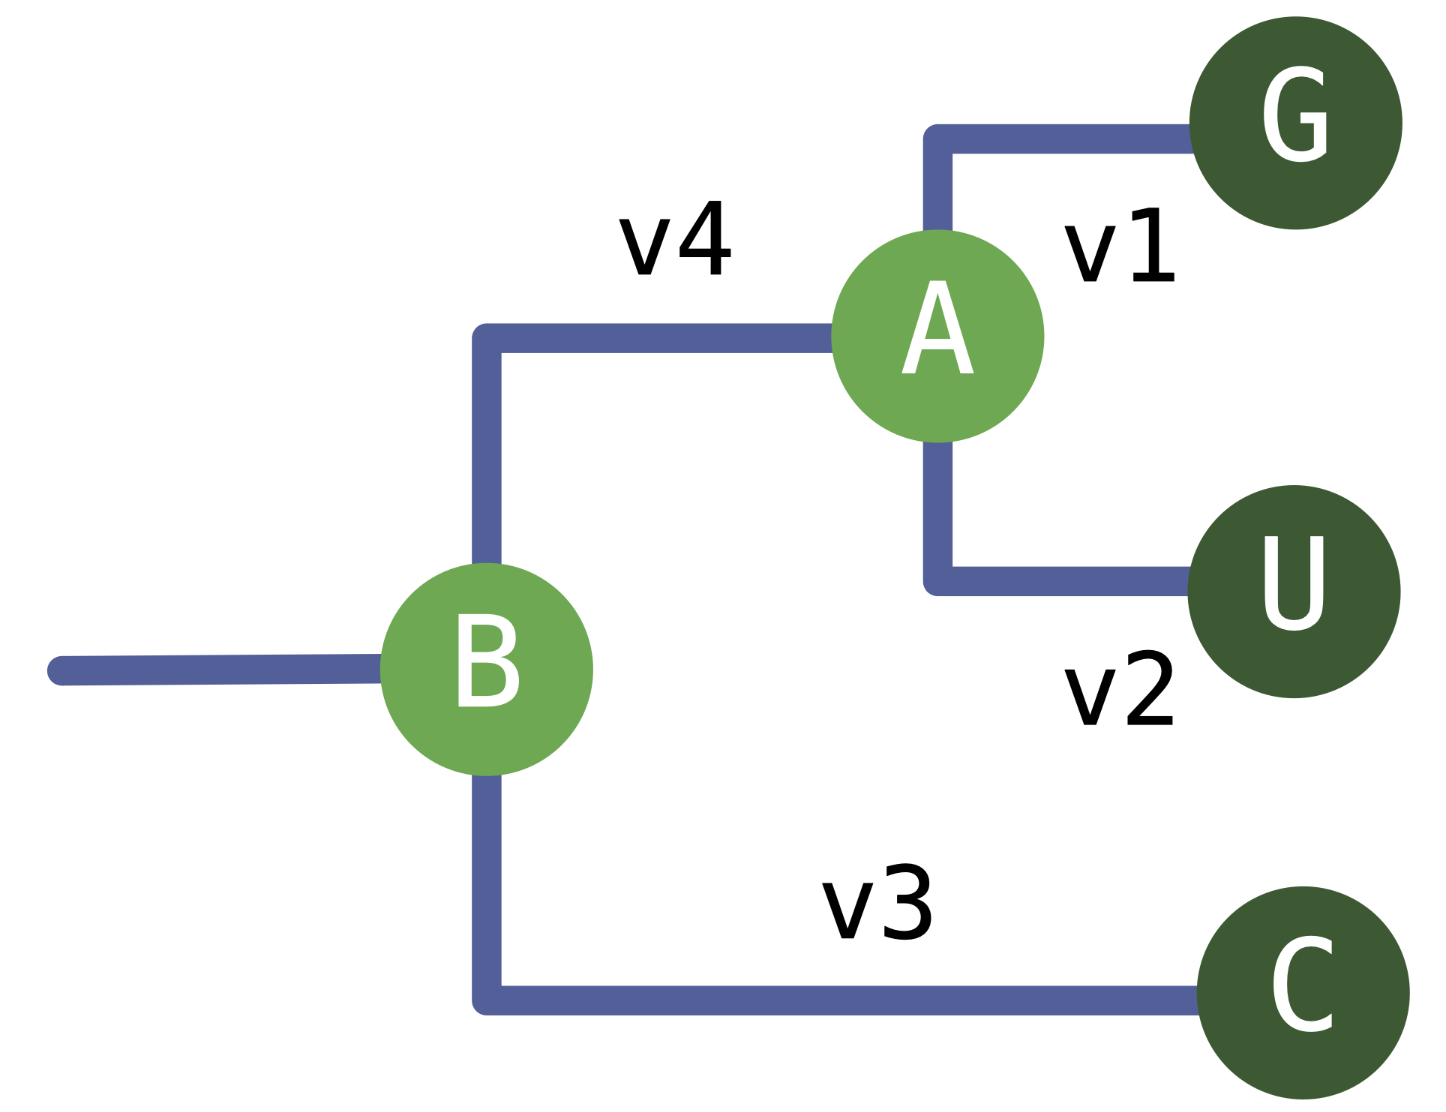
\includegraphics[width=0.34\textwidth]{images/phylogenetic_tree.png}
    \caption{A tree with nucleotides G, U and C at the tips; the interior states A and B are unknown.}
    \label{fig:tree}
\end{figure}

For the tree in Figure~\ref{fig:tree}, the probability of the tip states together with interior states $A, B$ is \cite{felsenstein1981}
$$P(\mathit{GUC}, AB) = \pi_A\, p_{AG}(v_1)\, p_{AU}(v_2)\, p_{AB}(v_4)\, p_{BC}(v_3),$$
where $p_{XY}(t)=[e^{Rt}]_{XY}$. The likelihood of the column sums over all interior states. Felsenstein's pruning algorithm computes this sum in time linear in the number of nodes. A gap is treated as an unknown nucleotide (a tip vector of all ones) \cite{knudsen2003}. We compute $\log P_{\text{single}}(i)$ for all columns and $\log P_{\text{pair}}(i,j)$ for all $n^2$ column pairs at once, as arrays of shape $n\times 4$ and $n\times n\times 16$. Every node is rescaled, so large alignments do not underflow.

\textbf{Tree.} The alignment tree has a neighbour-joining topology \cite{saitou1987} built from Jukes--Cantor distances. Its branch lengths are set by maximum likelihood under $R$: two sweeps of golden-section search per branch, using inside and outside partial likelihoods. The tree is then rooted at its midpoint. A PhyML tree \cite{guindon2010phyml} can be used instead.

\subsection{Gap-Bracket CYK}
Extending the grammar with the column evidence gives the Viterbi recursions below. All terms are log-probabilities, $q$ denotes rule probabilities, and $\rho_s$, $\rho_a$, $\rho_f$ are the \emph{start}, \emph{accelerate} and \emph{flag} ratios.
\begin{align*}
\mathrm{Pair}(i,j) &= M(i,j{-}1) + \log P_{\text{pair}}(i,j) + \chi(i,j)\log\rho_f\\
M(i,j) &= \log q_{\$M\to BF} + \max\big(F_{\text{st}}(i{+}1,j) + \log\rho_a,\\
&\qquad\qquad F_{\text{lp}}(i{+}1,j) + \log\rho_s\big)\\
F_{\text{st}}(i,j) &= \log q_{F\to \$M E} + \mathrm{Pair}(i,j)\\
F_{\text{lp}}(i,j) &= \log q_{F\to LS} + \max_k L(i,k) + S(k{+}1,j)\\
L(i,j) &= \log q_{L\to \$M E} + \mathrm{Pair}(i,j) \quad (i<j)\\
S(i,j) &= \max\big(\log q_{S\to \$M E} + \mathrm{Pair}(i,j),\\
&\qquad \log q_{S\to LS} + \max_k L(i,k) + S(k{+}1,j)\big)
\end{align*}
For a single column, $S(i,i) = \log q_{S\to s} + \log P_{\text{single}}(i)$, and likewise for $L$. The start ratio $\rho_s$ applies to a pair that closes a loop, i.e.\ the innermost pair of a helix. The accelerate ratio $\rho_a$ applies to a pair stacked on another pair, so $\rho_a > \rho_s$ favours long, uninterrupted helices. Because $F$ is split into its stacked and loop derivations, the ratios are applied exactly. The earlier implementation kept one $F$ cell, and the ratio depended on whichever derivation happened to score best there. $\chi(i,j)$ counts the first-pass pairs that cross $(i,j)$.

Each span length is filled with one vectorised array operation, so a pass costs $O(n^3)$ arithmetic but only $O(n)$ Python iterations. The recursions and traceback are tested against exhaustive enumeration of all structures on random inputs.

\textbf{First pass.} The parser runs on all columns ($\chi = 0$) and returns the nested structure, written with \texttt{()}.

\textbf{Second pass.} The first-pass pairs are removed. The parser runs again on the remaining columns, with its own $\rho_s, \rho_a$ and the crossing weight $\rho_f$, and the pairs it finds are written with \texttt{[]}. Repeating the procedure would find deeper pseudoknots.

\section{Parameters}
\subsection{Data}
Three Rfam families with a range of observed mutations define the evolutionary model and the grammar: RF00001 (5S rRNA), RF00005 (tRNA) and RF03000 (LOOT RNA motif). Three further families (RF01704, RF02035, RF03054) were tried early on and not used. The ratios are tuned on eight small validation families, and the method is evaluated on eight test families (Table~\ref{tab:families}). RF01737 appears in both sets, with different sequences, so we also report test scores without it. One validation reference, RF01722, contained an unmatched `\texttt{(}`, which we treat as unpaired.


\begin{table}[h]
\centering\footnotesize
\setlength{\tabcolsep}{2.5pt}
\begin{tabular}{llrr}
\toprule
\textbf{Set} & \textbf{Families} & \textbf{Seqs} & \textbf{Cols}\\
\midrule
Training & RF00001, RF00005, RF03000 & 368--954 & 118--230\\
Validation & RF01862, RF01834, RF01077, & 4--10 & 32--70\\
 & RF01090, RF01080, RF01722, & & \\
 & RF03537, RF01737 & & \\
Test & RF00556, RF00499, RF01084, & 3--25 & 33--191\\
 & RF03004, RF01089, RF01093, & & \\
 & RF01072, RF01737 & & \\
\bottomrule
\end{tabular}
\caption{Rfam families per set.}
\label{tab:families}
\end{table}

\subsection{Evolutionary parameters}
GC/CG pairs dominate stems (Table~\ref{tab:freq}), in line with their high stacking energy. Transitions (A$\leftrightarrow$G, C$\leftrightarrow$U) are faster than transversions (Table~\ref{tab:single}). In paired columns, changes that keep a pair canonical, such as UG$\to$CG or AU$\to$GC, are frequent, while changes that need two transversions are rare (Table~\ref{tab:pair}). Our re-implementation reproduces the parameters of the original notebooks to a relative difference of $10^{-4}$. The only difference is how ambiguous IUPAC symbols are handled.

\begin{table}[h]
\centering
\begin{tabular}{lr@{\qquad}lr}
\toprule
\multicolumn{2}{c}{\textbf{Paired bases}} & \multicolumn{2}{c}{\textbf{Single bases}}\\
\midrule
GC/CG  & 53.2\% & A & 37.2\% \\
AU/UA  & 30.8\% & C & 19.0\% \\
GU/UG  & 10.1\% & G & 18.7\% \\
Others & 5.9\%  & U & 25.1\% \\
\midrule
\textbf{Of positions} & \textbf{61.1\%} & \textbf{Of positions} & \textbf{38.9\%}\\
\bottomrule
\end{tabular}
\caption{Base frequencies in the three training families.}
\label{tab:freq}
\end{table}

\begin{table}[h]
\centering
\begin{tabular}{c|rrrr}
\toprule
\textbf{X / Y} & \textbf{A} & \textbf{C} & \textbf{G} & \textbf{U}\\
\midrule
\textbf{A} & $-0.44$ & 0.12 & 0.17 & 0.15 \\
\textbf{C} & 0.24 & $-0.77$ & 0.12 & 0.41 \\
\textbf{G} & 0.33 & 0.12 & $-0.62$ & 0.17 \\
\textbf{U} & 0.22 & 0.32 & 0.13 & $-0.66$ \\
\bottomrule
\end{tabular}
\caption{Single-base rate matrix $R$.}
\label{tab:single}
\end{table}

\begin{table}[h]
\centering
\setlength{\tabcolsep}{4pt}
\begin{tabular}{c|rrrrrr}
\toprule
\textbf{X / Y} & \textbf{AU} & \textbf{UA} & \textbf{GC} & \textbf{CG} & \textbf{UG} & \textbf{GU}\\
\midrule
\textbf{AU} & $-1.66$ & 0.28 & 0.68 & 0.21 & 0.03 & 0.25 \\
\textbf{UA} & 0.28 & $-1.66$ & 0.21 & 0.68 & 0.25 & 0.03 \\
\textbf{GC} & 0.37 & 0.11 & $-1.14$ & 0.24 & 0.03 & 0.26 \\
\textbf{CG} & 0.11 & 0.37 & 0.24 & $-1.14$ & 0.26 & 0.03 \\
\textbf{UG} & 0.10 & 0.76 & 0.16 & 1.47 & $-2.84$ & 0.03 \\
\textbf{GU} & 0.76 & 0.10 & 1.47 & 0.16 & 0.03 & $-2.84$ \\
\bottomrule
\end{tabular}
\caption{Entries of the paired rate matrix between canonical pairs (the diagonal also includes rates to non-canonical pairs).}
\label{tab:pair}
\end{table}

\subsection{Grammar parameters}
Relative rule frequencies in the nested part of the training structures:
\begin{align*}
    &S \rightarrow L\,S\ (88.4\%) \mid \$M\,E\ (2.3\%) \mid s\ (9.3\%)\\
    &F \rightarrow \$M\,E\ (61.6\%) \mid L\,S\ (38.4\%)\\
    &L \rightarrow \$M\,E\ (8.6\%) \mid s\ (91.4\%)\\
    &\$M \rightarrow B\,F\ (100\%) \qquad B, E \rightarrow d\ (100\%)
\end{align*}
The original notebooks estimated these with inside--outside on strings of paired/unpaired symbols, which gave similar values (88.6/1.9/9.5, 62.5/37.5, 8.7/91.3\%). That estimate does not know which bases pair with which, so we use the exact counts instead.

\subsection{Gap-Bracket ratios}
The ratios were chosen by grid search on the validation set, maximising pooled base-pair F1. The grid covered $\{0.25, 0.35, 0.5, 0.7, 1, 1.4, 2, 2.8, 4\}$ for $\rho_s,\rho_a$ and $\{0.25,\dots,2\}$ for $\rho_f$. The first pass was tuned alone, then the second pass on top of it, and ties went to the setting closest to 1. The whole search takes about 10 seconds. The genetic algorithm of the original notebooks needed an estimated several hours, because every evaluation re-ran PhyML and a dictionary-based parser.

\begin{table}[h]
\centering
\begin{tabular}{lccc}
\toprule
 & \textbf{Start} $\rho_s$ & \textbf{Accelerate} $\rho_a$ & \textbf{Flag} $\rho_f$\\
\midrule
\multicolumn{4}{l}{\textit{Grid search (this report, default)}}\\
1st pass & 0.35 & 2.00 & -- \\
2nd pass & 1.00 & 1.40 & 1.00 \\
\multicolumn{4}{l}{\textit{Genetic algorithm (2025 notebooks)}}\\
1st pass & 0.19 & 1.48 & -- \\
2nd pass & 0.88 & 1.78 & 0.98 \\
\bottomrule
\end{tabular}
\caption{Gap-Bracket ratios. Both searches find $\rho_s < 1 < \rho_a$ in the first pass: helices are cheap to extend and expensive to start.}
\label{tab:ratios}
\end{table}

\section{Results}
The main measure is pooled base-pair F1 over the families of a set. For continuity with the 2025 report we also give the \emph{weighted} score used there: pair F1 and unpaired-column F1 averaged with weights $2\times$(reference pairs) and (reference unpaired columns). Confidence intervals come from resampling families with replacement (10{,}000 resamples).

\begin{table}[h]
\centering
\setlength{\tabcolsep}{3.5pt}
\begin{tabular}{lcccc}
\toprule
\textbf{Model} & \textbf{P} & \textbf{R} & \textbf{F1} & \textbf{Wtd.}\\
\midrule
\multicolumn{5}{l}{\textit{Validation (8 families, used for tuning)}}\\
KH-99 CYK & .820 & .701 & .756 & .780\\
Gap-Bracket, 1st pass & .846 & .752 & .796 & .814\\
Gap-Bracket, 2 passes & .836 & .872 & \textbf{.854} & .866\\
\quad with 2025 GA ratios & .832 & .846 & .839 & .854\\
\midrule
\multicolumn{5}{l}{\textit{Test (8 held-out families)}}\\
KH-99 CYK & .748 & .604 & .669 & .703\\
Gap-Bracket, 1st pass & .770 & .731 & .750 & .750\\
Gap-Bracket, 2 passes & .769 & .843 & \textbf{.804} & .798\\
\quad with 2025 GA ratios & .793 & .858 & .824 & .818\\
\bottomrule
\end{tabular}
\caption{Pooled precision, recall, base-pair F1 and the legacy weighted score. KH-99 CYK is the same parser with all ratios equal to 1 and one pass.}
\label{tab:results}
\end{table}

Table~\ref{tab:results} and Figure~\ref{fig:families} summarise the results. On the test set, the first-pass ratios raise F1 from 0.669 to 0.750, mostly through recall: helices are no longer broken into fragments. The second pass adds 0.054 F1 (95\% CI 0.006--0.116) by recovering pseudoknotted helices, and raises recall to 0.843 with almost no loss of precision. Overall, the gain over KH-99 CYK is 0.135 (CI 0.007--0.331). Without the overlapping family RF01737, test F1 is 0.650, 0.743 and 0.803 for the three models.

The genetic-algorithm ratios score lower than the grid-search ratios on validation (0.839 vs 0.854) but higher on test (0.824 vs 0.804; difference CI 0.001--0.050). Tuning five ratios on eight small families overfits somewhat. Both settings were fixed on validation data, so we keep the grid-search ratios as the default rather than choosing between them by test score. With a benchmark this small, intervals are wide, and differences of a few F1 points should not be over-interpreted.

\textbf{Reproduction.} With PhyML trees and the genetic-algorithm ratios, as in the original notebooks, the new implementation gives a weighted test score of 0.817. The 2025 report gave 0.824, and four of the eight families (RF00556, RF00499, RF01072, RF01737) agree to within 0.1 points. The remaining differences come from the exact application of the ratios (Section~3.3), the crossing count over the full pair span, and the exact grammar counts.

\begin{figure*}[t]
    \centering
    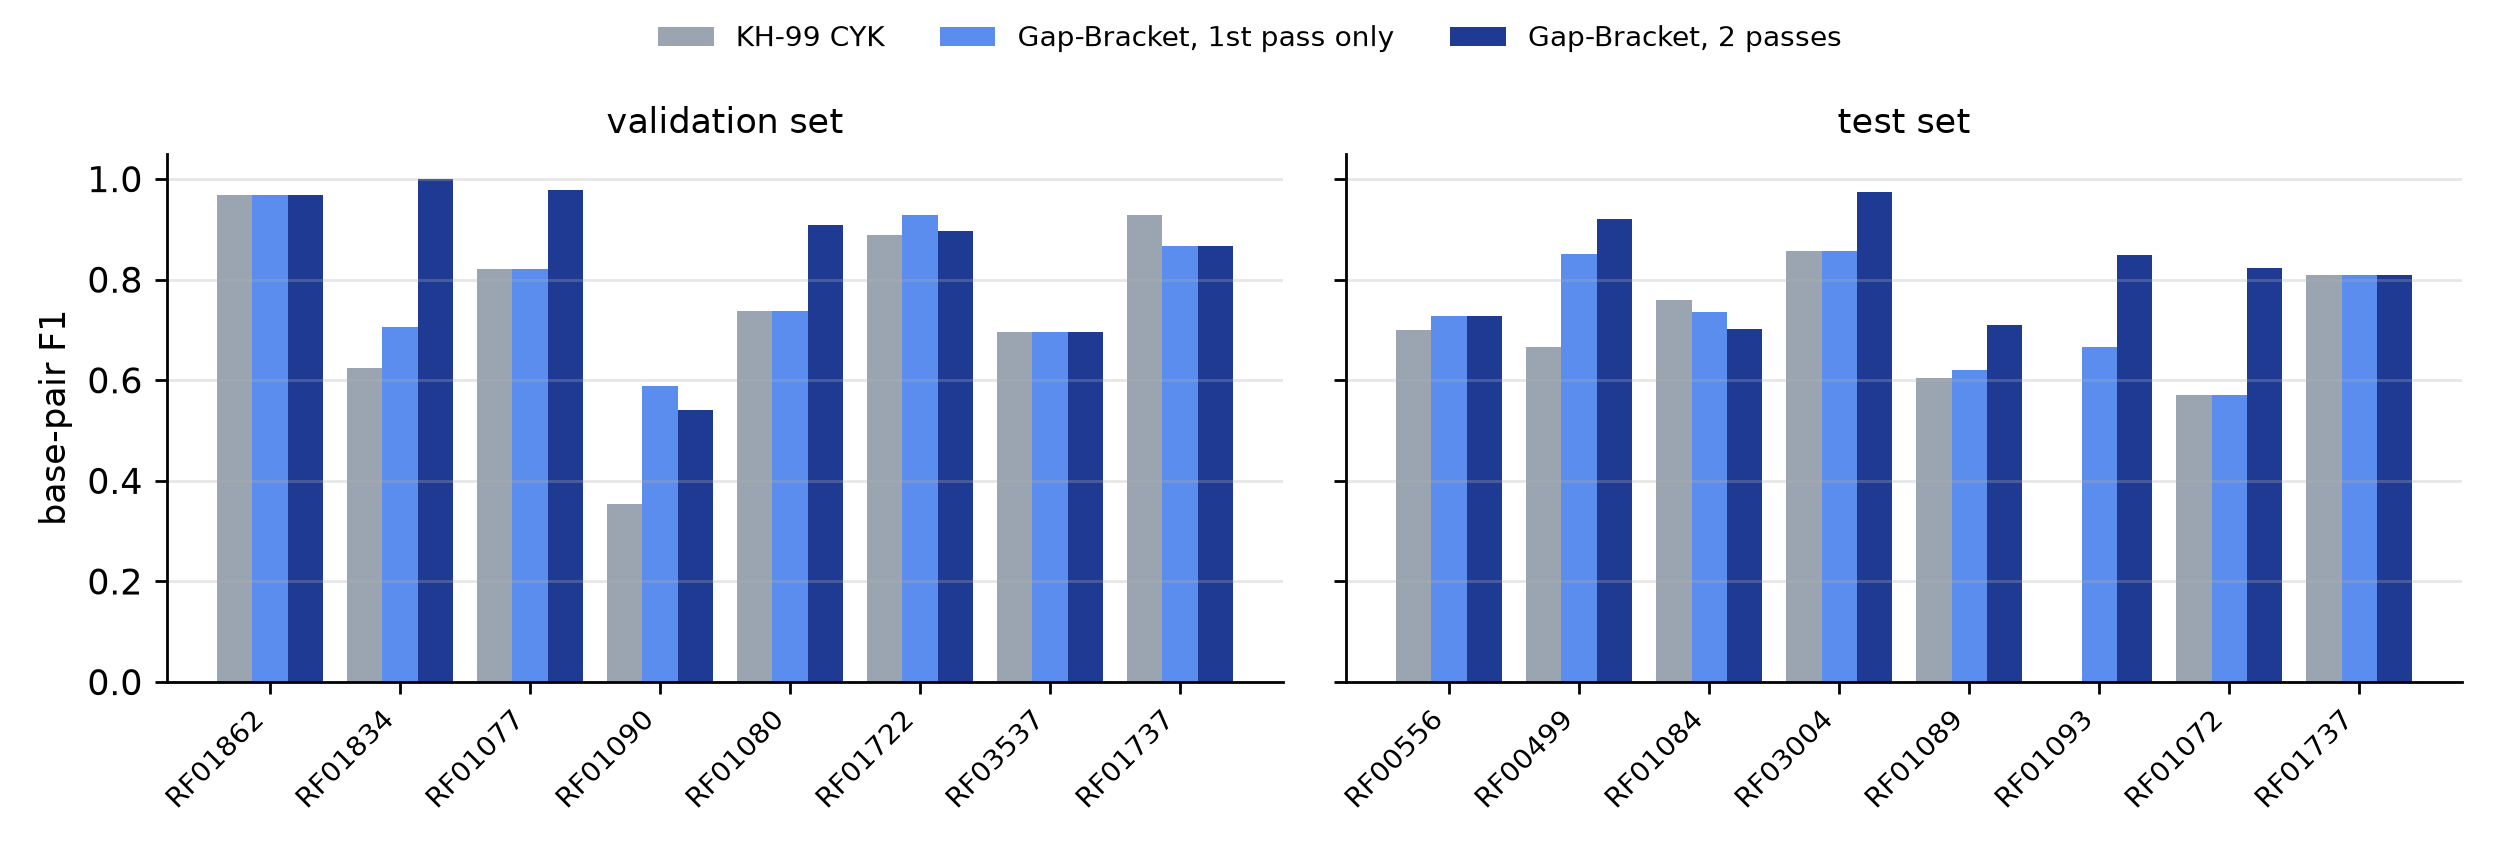
\includegraphics[width=0.9\textwidth]{images/family_f1.png}
    \caption{Base-pair F1 per family. The second pass mainly helps families with pseudoknots (RF01834, RF01077, RF01080, RF03004, RF01093, RF01072).}
    \label{fig:families}
\end{figure*}

\begin{table}[h]
\centering
\setlength{\tabcolsep}{4pt}
\begin{tabular}{lrrrr}
\toprule
\textbf{Family} & \textbf{Seqs} & \textbf{Cols} & \textbf{2025 code} & \textbf{This work}\\
\midrule
RF01737 & 3 & 68 & 3.3\,s & 10\,ms\\
RF01072 & 25 & 33 & 5.5\,s & 104\,ms\\
RF00556 & 10 & 46 & 6.5\,s & 40\,ms\\
RF01093 & 12 & 60 & 14.6\,s & 50\,ms\\
RF03004 & 9 & 84 & 27.8\,s & 41\,ms\\
RF00499 & 5 & 117 & 54.6\,s & 27\,ms\\
RF01089 & 7 & 134 & 736\,s & 44\,ms\\
RF01084 & 9 & 191 & $>$40\,min$^\dagger$ & 82\,ms\\
\bottomrule
\end{tabular}
\caption{Wall-clock time to predict one test alignment (tree, column likelihoods and both passes) on an Apple-silicon laptop. The 2025 code ran PhyML under Rosetta. $^\dagger$Stopped after 40 minutes.}
\label{tab:time}
\end{table}

\textbf{Speed.} Table~\ref{tab:time} compares running times. The original implementation wrote an extended grammar with one rule per distinct column pattern to disk, then ran a dictionary-based CYK over it, so its cost grew with both alignment length and the number of distinct columns. The new implementation computes all column likelihoods as arrays and fills each span length of the chart in a single vectorised step.

\section{Discussion}
Two failure modes remain.
\begin{enumerate}
    \item \textbf{Alignments unlike the training families.} The model is estimated from only three families. RF01084 (191 columns), for example, contains long, gappy regions. There, the pair evidence is weak and the grammar prefers short local helices.
    \item \textbf{Poorly conserved, gappy columns.} Gaps are unknown nucleotides, so a column that is filled in only one or two sequences can still support a pair. The structure of such a region then depends on very few sequences.
\end{enumerate}

\noindent RF00499 (first 54 columns) shows the effect of the first-pass ratios. KH-99 CYK breaks the long central helix into fragments, while the Gap-Bracket parser recovers most of it:

\begin{tcolorbox}[colback=green!5!white, colframe=green!30!black, title=RF00499, fontupper=\ttfamily\scriptsize, left=2pt, right=2pt]
Ref\ \ ...((((((((((((((((((((((((((.((((((........))))))..)) \\
KH99 ...(((((((...........((((.....((((((........)))))).... \\
GB\ \ \ ...(((((((.((((((((((((((((((.((((((........))))))..))
\end{tcolorbox}

\noindent RF01084 (first 54 columns) shows the gap problem. The first 38 columns are present in only one of nine sequences, yet both parsers place helices there, and the Gap-Bracket parser even predicts spurious crossing pairs:

\begin{tcolorbox}[colback=green!5!white, colframe=green!30!black, title=RF01084, fontupper=\ttfamily\scriptsize, left=2pt, right=2pt]
Ref\ \ ......................................(((((((..((((((. \\
KH99 .(((((.....)))))....(((((..)))))......(((((((..(((((.. \\
GB\ \ \ [((((([[...)))))(((((((((..))))).)))).(((((((..((((((.
\end{tcolorbox}

Clustering families and training a model per cluster could address the first issue. For the second, pairs could require a minimum number of sequences with bases in both columns, or the column likelihood could be weighted by how many sequences are gap-free there.

\section{Conclusion}
The model rests on three assumptions: stems tend to be long and adjacent; whether a pair starts or extends a helix changes its probability; and pseudoknotted helices can be found once the nested structure is fixed. The start and accelerate ratios express the first two, and the two-pass parser expresses the third. On held-out families they raise base-pair F1 from 0.669 (KH-99 CYK) to 0.804. The clean implementation makes the method fast enough to tune and evaluate in seconds. With that in place, the next steps are a larger benchmark, more training families, and loop-length-dependent grammar parameters.

\bibliographystyle{abbrv}
\bibliography{references}

\end{document}
